\Chapter{A probléma és az eszközkészlet bemutatása}

\Section{Online foglalás}

Az online szállásfoglaló oldalak megjelenésével egyszerűsődött a turisták dolga, hiszen egyszerre rengeteg szálláshelyhez hozzáfértek egy platformon. Láthatták a különböző árakat, milyen szolgáltatásai vannak egyes helyeknek, és hogy hol található. A szállodáknak is egyszerűbb lett a dolga, hiszen nincs más dolga, minthogy szállását feltölti a különféle oldalakra, és mivel ezeknek általában hatalmas a látogatottsága, máris több millió ember számára vált láthatóvá. Eltérő ajánlatokat tehet fel, amivel kedvezőbbé válhat a vendégek számára, mint a konkurencia.

A hátulütője a dolognak a szállásadó részéről, hogy foglalást akármilyen fizetési kötelezettség nélkül véghez vihet a vendég, ugyanez igaz a lemondásra is. Van lehetősége a szállás tulajdonosának, csak úgy engedélyezni az online foglalást, hogy a foglalónak kötelező bankkártyát megadni, és a foglalás összegének egy bizonyos részét le is vonhatja. Azonban ebben az esetben lehetséges, hogy a vendégek más hotelt fognak keresni az online felületen, ahol nem kell ilyen adatokat megadni ezáltal potenciális ügyfelektől fosztja meg magát a szálloda.

Egy tanulmány szerint ami a \ref{fig:lemondasi}\cite{online_lemondas} ábrán látható az online foglalások 40\% lemondásra kerül. 2014-ben az átlagos lemondási arány 32.9\% volt. 2018-ban azonban már elérte a 39.6\%-ot\cite{online_lemondas}.

\begin{figure}[h]
    \caption{Lemondási arányok évekre lebontva}
    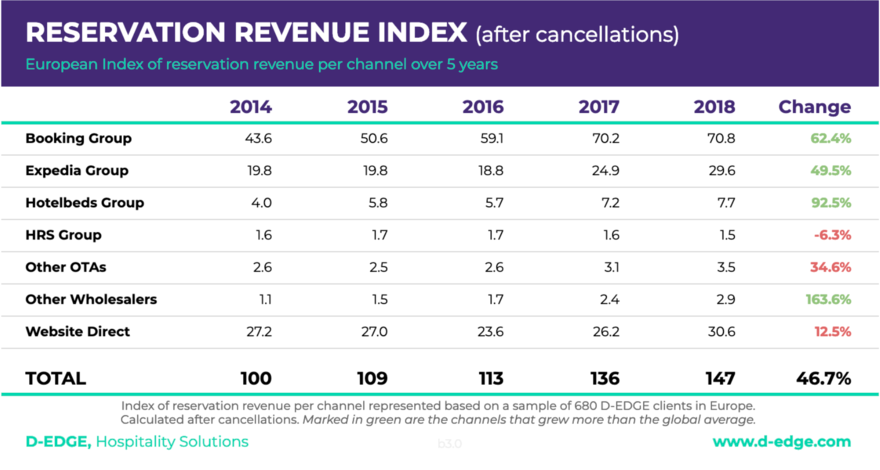
\includegraphics[scale=0.45]{images/2.fejezet/Online_foglalas_lemondas_szazalek.png}
    \label{fig:lemondasi}
\end{figure}  
Ezek az online közvetítő oldalak arra ösztönzik a turistákat, hogy minél többet és többet foglaljanak, hiszen ha le szeretnék mondani a foglalást azt minden következmény nélkül megtehetik. Ez több gonddal is jár a szállásadónak \cite{online_lemondas}.
\begin{itemize}
    \item Bevételt veszítenek ha a lemondott foglalás után nem tudják eladni a szobát.
    \item Úgynevezett last minute árcsökkentést kell bevetni azért, hogy eladják a szobát. Ezzel is bevételt veszít a szálloda hiszen lehet, hogy az előző nap még teljes áron is eltudták volna adni.
    \item A bevétel kiesést elkerülve eladhat több szobát a szálláshely mint amennyi a rendelkezésre áll, ezzel azonban megkockáztatja azt, hogy ha nem mondanak le foglalást valamelyik vendégnek nem fog szoba jutni.
\end{itemize}

A modell, amit a szakdolgozatom során építeni fogok, erre a problémakörre kínál megoldást nyújtani. Ezzel ugyanis egyszerűbb lesz megmondani, hogy melyik szobákat fogják lemondani, ezeket a szobákat célszerű lehet még egyszer eladni, csökkentve ezzel annak a valószínűségét, hogy nem sikerül eladni a szobát egy lemondás után, vagy hogy a szoba árát last minute csökkenteni kell az eladás reményében.


\Section{Használt technológiák}

Ebben a fejezetben a szakdolgozatomban használt különböző technológiákról, programozási nyelvekről, könyvtárakról és eszközökről fogok írni. Arról mi mire való, mit hogyan használtam az adatelemzés és modell építés során.

Az elemzés és modell építés során használt technológiák és nyelvek az alábbiak.
\begin{itemize}
\item Python: a programozás nyelv amivel, különböző notebook-okban dolgoztam.
\item Jupyter Notebook: különböző notebook-ok létrehozására, ahová a programot írtam.
\item Numpy: egy kiegészítő csomag amivel több dimenziós tömböket és mátrixokat tudunk kezelni.
\item Pandas:  egy Python progamkönyvtár, ami az adatokkal való különböző műveleteket könnyíti meg.
\item Matplotlib: egy ábrázolási könyvtár.
\item Seaborn: egy könyvtár statisztikai grafikák készítésére.
\item Scikit-learn: egy ingyenes gépi tanulási könyvtár a Python programozási nyelvhez.
\end{itemize}

A következő szakaszokban ezek kerülnek részletezésre.

\subsection{Python}
A Python egy általános célú, nagyon magas szintű programozási nyelv, melyet Guido van Rossum holland programozó kezdett el fejleszteni 1989 végén, majd hozott nyilvánosságra 1991-ben. A nyelv tervezési filozófiája az olvashatóságot és a programozói munka megkönnyítését helyezi előtérbe a futási sebességgel szemben.

A Python többek között a funkcionális, az objektumorientált, az imperatív és a procedurális programozási paradigmákat támogatja. Dinamikus típusokat és automatikus memóriakezelést használ, ilyen szempontból hasonlít a Scheme, Perl és Ruby nyelvekhez, emellett szigorú típusrendszerrel rendelkezik.

A Python úgynevezett interpreteres nyelv, ami azt jelenti, hogy nincs különválasztva a forrás- és tárgykód, a megírt program máris futtatható, ha rendelkezünk a Python értelmezővel. A Python értelmezőt számos géptípusra és operációs rendszerre elkészítették, továbbá számtalan kiegészítő könyvtár készült hozzá, így rendkívül széles körben használhatóvá vált \cite{python}.

\subsection{Jupyter Notebook}
Az egész egy projekt, aminek a célja egy nyílt forráskódú, nyílt szabványok és szolgáltatások fejlesztése interaktív fejlesztési feladatokra több programozási nyelv elérhetőségének biztosításával.

Ebből fejlődött ki a Jupyter Notebook, ami egy webalapú interaktív fejlesztési környezet amivel, Jupyter Notebook dokumentumokat lehet létrehozni. Valójában ez a dokumentum egy JSON formátumban lévő fájl, ami egy rendezett listát tartalmaz az input és output cellákról. Ezek a cellák tartalmazhatnak kódot, szöveget Markdown segítségével, matematikai számításokat, különböző ábrázolásokat és média fájlokat. A munkafüzet kiterjesztése általában ".ipynb" \cite{project_jupyter}.

\begin{figure}[h!]
    \centering
    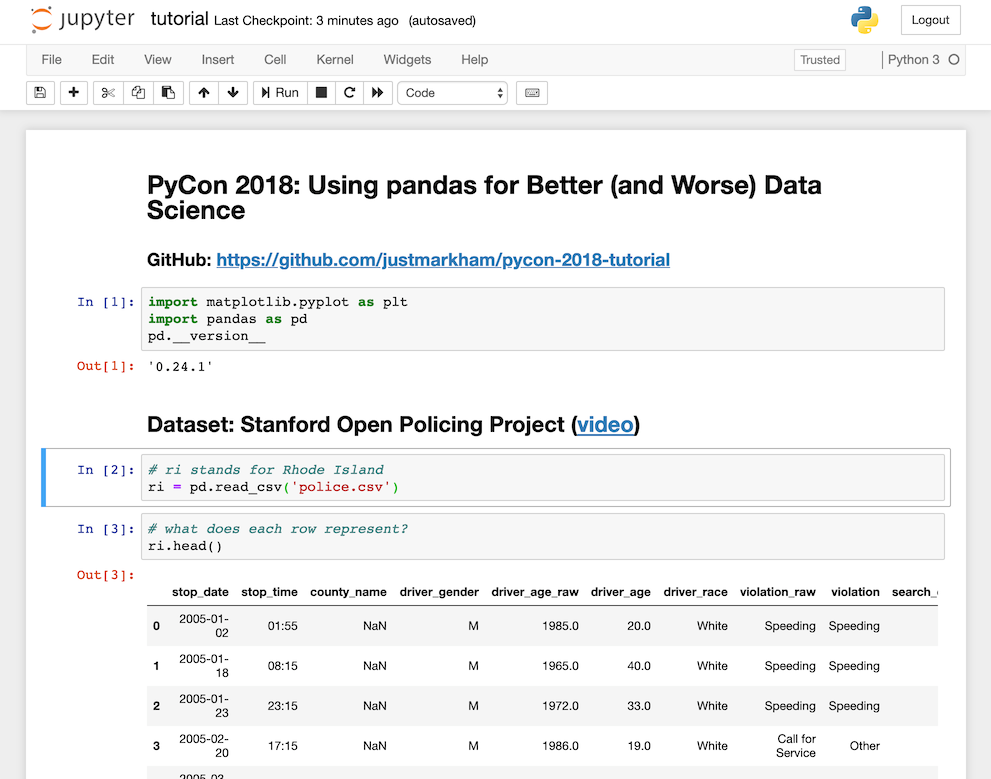
\includegraphics[scale=0.6]{images/2.fejezet/jupyter_notebook.png}
    \caption{Jupyter notebook kinézete}
    \label{fig:my_label}
\end{figure}

\subsection{Numpy}
A NumPy nyílt forráskódú kiegészítő csomag a Python programozási nyelvhez, mely a nagy, többdimenziós tömbök és mátrixok használatát támogatja egy nagy magas szintű matematikai függvénykönyvtárral. A Python programozási nyelv eredetileg nem numerikus számításokra volt tervezve, de még a tervezés elején felkeltette a kutató- és mérnökközösség figyelmét. 2006-ban a Numarray és a Numeric csomagokból – a SciPy projekt részeként – létrejött a NumPy v1.0, hogy a SciPy csomag ne legyen túl nagy, a NumPy-t külön csomagként adták ki \cite{numpy}.

\subsection{Pandas}
A pandas a Python programozási nyelv egyik progamkönyvtára, amely adatok feldolgozására és elemzésére szolgál. Különösen adattáblák és idősorok. feldolgozásához szolgáltat megfelelő adatszerkezeteket. Ez a szabad szoftver a három-záradékos BSD licenc alatt jelent meg.

A könyvtár néhány funckiója:
\begin{itemize}
    \item DataFrame objektum az adat feldolgozására indexelési lehetőséggel,
    \item az adatok igazítását, valamint a hiányzó adatok kezelése,
    \item adathalmazok átalakítása és pivot táblába rendezése,
    \item oszlopok beillesztése, törlése.
\end{itemize}

A könyvtár teljesítményét úgy optimalizálják, hogy a kritikus kódokat Cython vagy C nyelven írják meg \cite{pandas}.

\subsection{Matplotlib}
Egy ábrázolási könyvtár a Python programozási nyelvhez és a Numpy kiegészítőhöz. Egy objektum orientált alkalmazásprogramozási felületet biztosít függvények beágyazására különböző alkalmazásokba. Eredeti kódot John D. Hunter írta, azóta azonban egy aktív fejlesztői közösség fejleszti a BSD licenc alatt. A Matplotlib úgy van tervezve, hogy a MATLAB-éhoz hasonló grafikonokat lehessen készíteni Python nyelven. Annyi különbséggel, hogy a Matplotlib ingyenes és nyílt forráskódú \cite{matplotlib}.

\subsection{Seaborn}
A Matplotlib-hez hasonlóan ezzel a könyvtárral is grafikonokat, függvényeket tudunk ábrázolni. A Matplotlib-re építették az egészet és a Pandas könyvtárban megtalálható adatstruktúrákkal szorosan integrálva van. A Seaborn lényege, hogy a vizualizációt egy központi részéve tegye az adatok felfedezésének és megértésének \cite{seaborn}.

\subsection{Scikit-learn}
A Python programozási nyelvhez fejlesztett gépi tanulási könyvtár. Különböző osztályozási, regressziós és klaszterezési modellek találhatóak benne. A könyvtárt David Cournapeau hozta létre egy Google rendezvény projektjeként. 2010-ben Fabian Pedregosa, Gael Varoquaux, Alexandre Gramfort és Vincent Michel átvették a projektben a vezető szerepet és ugyanezen év február elsején kiadták az első nyilvános kiadást. A fentebb említett könyvtárak közül többel is kiválóan van integrálva, mint például a Matplotlib, Numpy, Pandas. Ez az egyik legnépszerűbb gépi tanulással foglalkozó könyvtár a Github-on \cite{scikit-learn}.

\Section{Gépi tanulás}
A dolgozatom nagy része a gépi tanulással foglalkozik, de mi is ez valójában? Ebben a fejezetben ezt szeretném elmagyarázni.

A gépi tanulás matematikai adatmodellekkel tanít be számítógépeket közvetlen felügyelet nélkül. Ez a mesterséges intelligencia egy részhalmaza. A gépi tanulás algoritmusokkal azonosít mintákat az adatokban, amelyekkel ezután adatmodellt készít, és előrejelzéseket végez. A gépi tanulás eredményei az adatok és a tapasztalat mennyiségének növekedésével várhatóan egyre pontosabbak \cite{machinelearningbasics}.

\subsection{A gépi tanulás előnyei}
Mivel rengeteg helyen és helyzetben lehet használni, ezért most csak néhányt előnyt sorolnék fel a teljesség igénye nékül.
\begin{itemize}
    \item Feltáró elemzés: A gépi tanulással azonosítható mind a strukturált, mind a strukturálatlan adatokban rejlő minta vagy szerkezet, így könnyebben látható, mit is mutatnak az adatok.
    \item Ügyfelek viselkedésének előrejelzése: A gépi tanulással ügyfélhez kapcsolódó adatok bányászhatók, amelyekkel könnyebben azonosíthatók minták és viselkedésmódok, ami optimalizált termékjavaslatokat és a lehető legjobb vásárlói élményt eredményezheti. Ez az a része a gépi tanulásnak amit a szakdolgozatomba megfogunk vizsgálni, hogy egy adott ügyfél lemondja-e vagy sem a szállást.
    \item A felhasználói élmény fejlesztése: Adaptív interfészek, célzott tartalom, csevegőrobotok, hangvezérelt virtuális asszisztensek – ezek mind példák arra, hogy a gépi tanulás hogyan segíthet optimalizálni az ügyfélélményt\cite{machinelearningbasics}.
\end{itemize}

\subsection{A gépi tanulás lehetséges technikáinak egy tipikus besorolása az alábbi.}
\begin{itemize}
    \item Felügyelt tanulás: Címkékkel vagy struktúrával ellátott adatkészletek esetén az adatok „betanítják” a gépet, így az hatékonyabban végezhet előrejelzéseket és hozhat döntéseket \cite{machinelearningbasics}. Például megadhatunk egy adatkészletet, amely az elmúlt 100 évre vonatkozóan városok népességi adatait tartalmazza, és azt szeretnénk tudni, hogy egy adott város népessége hogyan alakul majd négy év múlva. Az eredmény olyan címkéket használ, amelyek már szerepelnek az adatkészletben: népesség, város és év \cite{machinelearningalgorithms}.
    \item Felügyelet nélküli tanulás: Adatok klaszterekbe való csoportosításával könnyebben foglalkozhat címkék vagy struktúra nélküli adatokkal, valamint azonosíthat mintákat és kapcsolatokat \cite{machinelearningbasics}. Például megadjuk az ügyféladatokat, és olyan ügyfélcsoportokat szeretnénk eredményül kapni, akik hasonló termékeket kedvelnek. Az általunk megadott adatok nincsenek megcímkézve, és az eredményben szereplő címkék az adatpontok között felderített hasonlóságok alapján jönnek létre \cite{machinelearningalgorithms}.
    \item Megerősítő tanulás: A megerősítéses tanulás nem támaszkodik a címkézett adatkészletekre, itt a modellnek nem mondjuk meg, hogy mely műveleteket kell végrehajtania, vagy épp a feladat optimális végrehajtásának módját. A megerősítéses tanulásnál jutalmakat és büntetéseket használunk az egyes döntésekhez kapcsolódó címkék helyett annak jelzésére, hogy a megtett művelet jó vagy rossz \cite{reinforcementlearning}. Tegyük fel például, hogy önvezető autót tervezünk, és biztosítani szeretnénk, hogy az autó betartja a szabályokat, és az emberek biztonságáról is gondoskodik. Amint az autó tapasztalatokat szerez és már vannak megerősítő előzményei, megtanulja, hogyan maradhat a saját sávjában, hogyan tarthatja tiszteletben a sebességkorlátozást, és hogy fékezzen ha gyalogost lát\cite{machinelearningalgorithms}.
\end{itemize}

\subsection{A megoldandó feladatokat szintén kategorizálni szokták.}
\begin{itemize}
    \item Osztályozás: A bemenetek két vagy több osztályra oszlanak, amik címkézve vannak. Az algoritmusnak olyan modellt kell létrehoznia, amely képes osztályokba sorolni a különböző adatok által meghatározott bemeneteket. Az ilyen típusú feladatokat általában felügyelt tanulási módszerrel oldják meg. Például egy képről meghatárázni, hogy kutya vagy macska található rajta. Ez látható a \ref{fig:osztalyozas} ábrán.
    \item Regresszió: Hasonló az osztályozáshoz azzal a különbséggel, hogy a kimenetnek folyamatos tartománya van. A bemenetek itt is címkézve vannak. Általában ezt is felügyelt tanulással valósítják meg. Ilyen feladat lehet a részvények árának meghatározása. Ez látható a \ref{fig:regresszio} ábrán.
    \item Klaszterezés: Olyan adatokat csoportokba szedni amik nincsenek címkézve, úgy hogy az adott csoporton belüli elemek hasonlósága a legnagyobb legyen és egymástól minél jobban elkülöníthető csoportokat kapjunk. Például spam email-ek megjelölésére használható. Ez látható a \ref{fig:klaszterezes} ábrán.
\end{itemize}
\begin{figure}[h]
    \centering
    \begin{subfigure}{0.3\textwidth}
        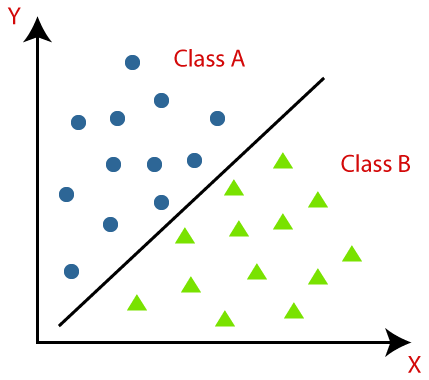
\includegraphics[width=0.8\linewidth]{images/2.fejezet/osztalyozas.png} 
        \caption{Osztályozás}
        \label{fig:osztalyozas}
    \end{subfigure}
    \begin{subfigure}{0.3\textwidth}
        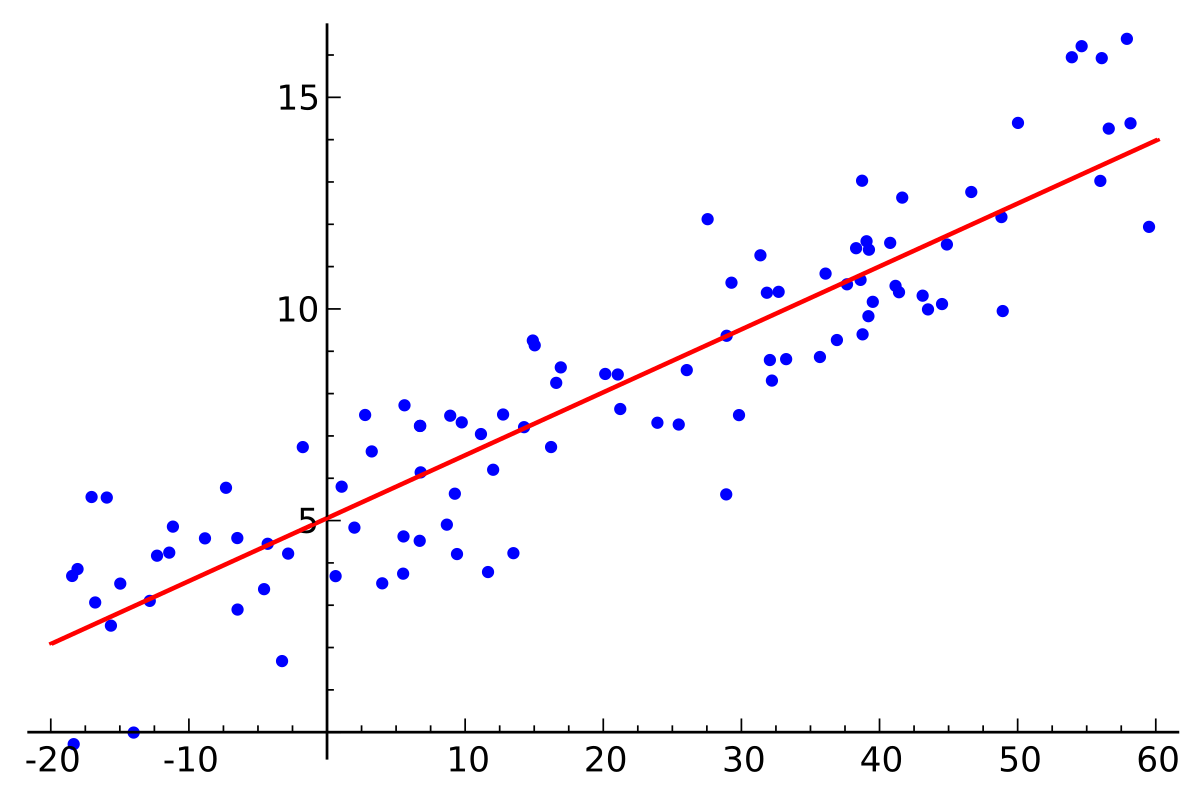
\includegraphics[width=1\linewidth]{images/2.fejezet/regresszio.png}
        \caption{Regresszió}
        \label{fig:regresszio}
    \end{subfigure}
    \begin{subfigure}{0.3\textwidth}
        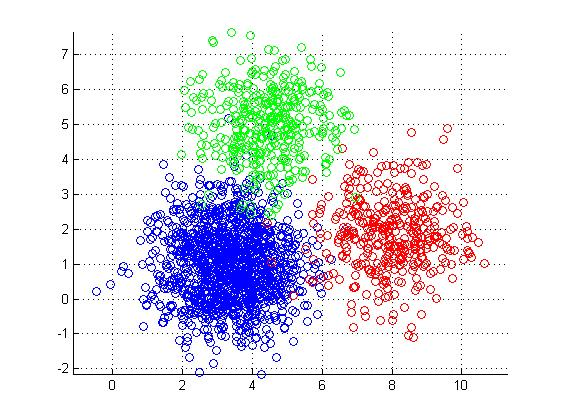
\includegraphics[width=1\linewidth]{images/2.fejezet/klaszterezes.jpg}
        \caption{Klaszterezés}
        \label{fig:klaszterezes}
    \end{subfigure}
    
    \caption{Gépi tanulás különféle feladatai képekkel szemléltetve}
\end{figure}

\Section{Gépi tanulás a szállodaiparban}
A mesterséges intelligencia és a gépi tanulás rengeteg iparágat befolyásolt. A szállodaiparban jobbá teszi a szolgáltatásokat azáltal, hogy személyre szabja a vendégek kiszolgálását, a fogyasztói viselkedést átláthatóvá teszi és meg tudja jósolni a vásárlási szokásokat és a jövőbeni trendeket. Az ajánló rendszerek múltbeli adatokat használnak, hogy információt szűrjenek ki és mintákat fedezzenek fel. Ezzel lehetőséget adva a viselkedések megvizsgálásának és előrejelzésének. Ezeket az adatokat használva ajánlhat szállodákat a látogatóknak. A vendégek akár elektornikus terminálon is be tudnak jelentkezni némelyik szálláshelyre, amin a háttérben futó gépi tanulási algoritmusok osztják ki a szobákat többféle kritérium alapján, ilyenek a tartozkódás hossza, a leendő érkezések, a szoba felszereltsége, a vendég típusa valamint, hogy visszatérő vendég-e.

Az online utazási irodák, mint a Booking.com, Expedia, TripAdvisor lehetőséget biztosítanak a szálláshelyek értékelésére. A szobák eladásának és az értékeléseknek szoros kapcsolata van. Egy felmérés megállapította, hogy a szálloda értékelése és a válasz a szállodától a negatív bírálatra az egyik legjobb előrejelzés, hogy az adott szálloda milyen jól teljesít pénzügyileg. A vendégek minősítéseiből fejlődhet egy szálloda, hogy jobbá tegye az élményt az ott tartozkodók számára. Azonban a hozzászólásokat átnézni egy embernek rengeteg idő, és nem is egyszerű feladat. A gépi tanulás segítségével ez is automatizálható, az algoritmusok kibányászak a szükséges információkat és klaszterezik ezeket ezzel segítve a vezetők munkáját. Számos megfigyelés igazolja, hogy az online értékelések befolyásolják a lehetséges szállóvendégeket azzal kapcsolatban, hogy melyik hotelt választják.

Több szálloda vezetője is úgy látja, hogy a gépi tanulás alkalmazása a fogyasztói szokások megértéséhez fokozta a vendégek elégedettségét és hűségét az adott szállodához. Egy 4 csillagos szálloda Portugáliában 39.000.000 euró bevételt mentett meg foglalások lemondásának előrejelzésével gépi tanulás segítségével.

A szállodák a bevételkezelésnél is használhatnak gépi tanulást. A szállodaipar a forgalmának 20\%-át elveszíti a lemondások miatt. A kereslet előrejelzés vagy foglalások lemondásának előrejelzésnél kulcsfontosságú a modell pontossága.

\begin{figure}[hbt!]
    \centering
    \caption{Különböző gépi tanulási feladatok a szállodaiparban}
    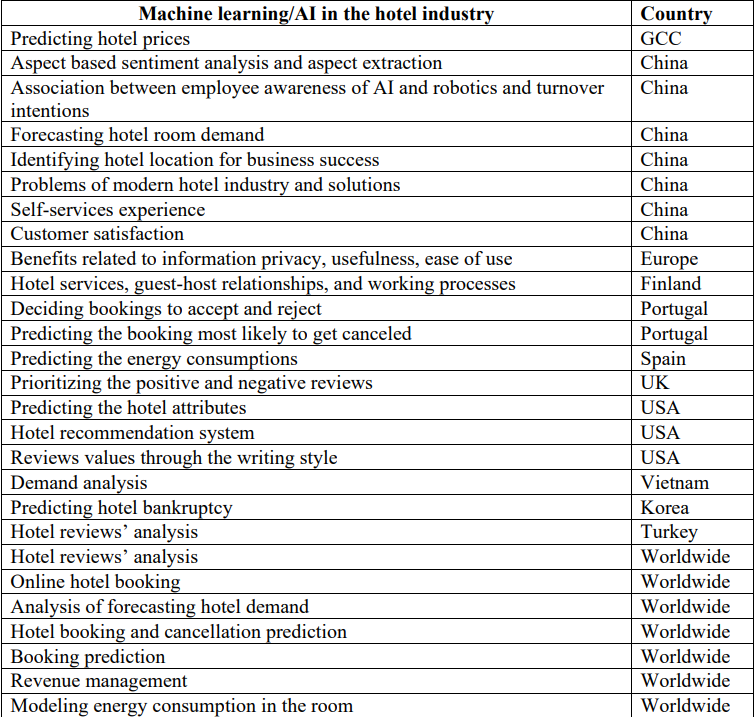
\includegraphics[scale=0.53]{images/2.fejezet/Gepi_tanulas_szallodaipar.PNG}
    \label{fig:gepitanulasszallodaiparban}
\end{figure}

A \ref{fig:gepitanulasszallodaiparban} táblázatban azt láthatjuk, hogy a szállodaipar milyen különféle részeit melyik országban vizsgálják és fejlesztik gépi tanulás segítségével. Láthatjuk, hogy az előbbi néhány példánál, mint a foglalás előrejelzés, visszajelzések elemzése vagy a vendégek viselkedésének meghatározásánál nem áll meg a dolog. Olyan problémák megoldására is használják, mint egy leendő hotel helyének meghatározása üzleti sikersség szempontjából vagy az energiafogyasztás megbecsülésére, milyen foglalásokat fogadjanak el vagy utasítsanak vissza.

Azonban azt láthatjuk, hogy a legnagyobb érdeklődést kiváltó fejlesztések a bevételkezeléssel vannak összefüggésben. Ezért is választottam szakdolgozatom témájának egy olyan modell építését, ami minél nagyobb pontossággal meg tudja határozni, hogy melyik foglalások lesznek lemondva \cite{gepi_tanulas_szallodaipar}.